\chapter{Algebraische Strukturen}
\begin{definition}{Magma}
	Eine Menge $M$ mit einer Verknüpfung $\star$ heißt \emph{Magma}, falls sie unter dieser Verknüpfung abgeschlossen ist, das heißt:
	\begin{equation*}
	  \forall u,v \in M: u\star v\in M
	\end{equation*}
\end{definition}

\begin{definition}{Halbgruppe}
	Eine Menge $M$ mit einer Verknüpfung $\star$ heißt \emph{Halbgruppe}, falls sie ein Magma ist und die Verknüpfung assoziativ ist:
	\begin{description}
	  \item[HG 1] $\forall u,v \in M: u\star v\in M$
	  \item[HG 2] $\forall u,v,w \in M: u\star(v\star w)=(u\star v)\star w$
	\end{description}
\end{definition}

\begin{definition}{Monoid}
	Eine Menge $M$ mit einer Verknüpfung $\star$ heißt \emph{Monoid}, falls sie eine Halbgruppe ist und ein neutrales Element bezüglich der Verknüpfung existiert:
	\begin{description}
	  \item[M 1] $\forall u,v \in M: u\star v\in M$
	  \item[M 2] $\forall u,v,w \in M: u\star(v\star w)=(u\star v)\star w$
	  \item[M 3] $\exists e \in M \quad \forall u\in M: e\star u=u\star e = u$
	\end{description}
\end{definition}

\begin{definition}{Gruppe}
	Eine Menge $G$ mit einer Verknüpfung $\star$ heißt \emph{Gruppe}, falls sie ein Monoid ist und zu jedem Element ein Inverses bezüglich der Verknüpfung exisitert:
	\begin{description}
	  \item[G 1] Die Verknüpfung assoziativ ist,
	  \item[G 2] ein neutrales Element besitzt,
	  \item[G 3] jedes Element invertierbar ist.
	\end{description}
	Falls die Verknüpfung zusätzlich kommutativ ist, nennt man die Gruppe eine \emph{abel'sche Gruppe} oder auch kommutative Gruppe.
\end{definition}

\par

\paragraph{Kurzübersicht} über die Strukturen Magma bis Gruppe, die Struktur sei jeweils $(M,\star)$
\begin{center}
		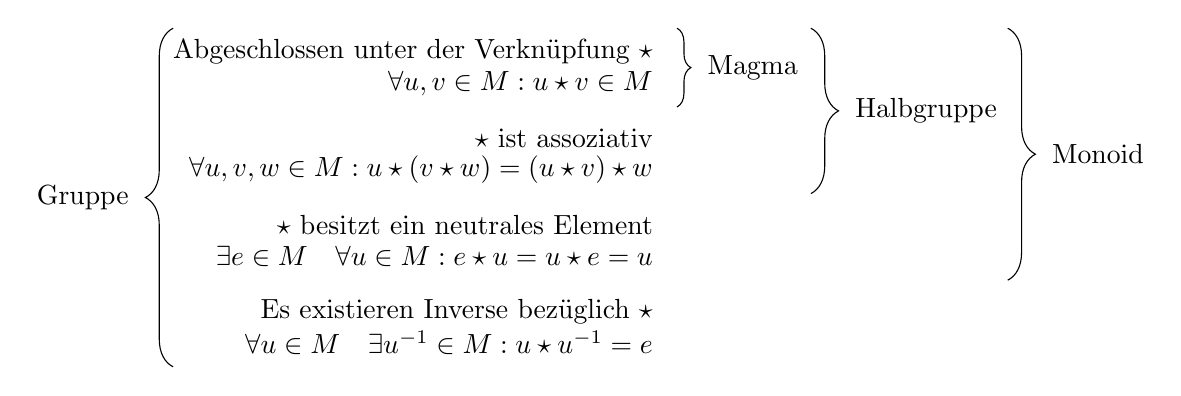
\begin{tikzpicture}
			\tikzset{
				grouplabel/.style={
					draw,
					fill = white,
					rectangle,
					inner sep = 4pt,
					rounded corners=1pt
				}
			}

		\draw node at (0,3.7) [label={left:Abgeschlossen unter der Verknüpfung $\star$}] {};
		\draw node at (0,3.3) [label={left:$\forall u,v \in M: u\star v\in M$}] {};

		\draw node at (0,2.6) [label={left:$\star$ ist assoziativ}] {};
		\draw node at (0,2.2) [label={left:$\forall u,v,w \in M: u\star(v\star w)=(u\star v)\star w$}] {};

		\draw node at (0,1.5) [label={left:$\star$ besitzt ein neutrales Element}] {};
		\draw node at (0,1.1) [label={left:$\exists e \in M \quad \forall u\in M: e\star u=u\star e = u$}] {};

		\draw node at (0,0.4) [label={left:Es existieren Inverse bezüglich $\star$}] {};
		\draw node at (0,0) [label={left:$\forall u\in M\quad\exists u^{-1}\in M:u\star u^{-1}= e $}] {};


		\draw [decorate,decoration={brace,amplitude=5pt},xshift=-4pt,yshift=0pt] (0.2,4) -- (0.2,3) node [black,midway,xshift=4pt,label={right:Magma}] {};

		\draw [decorate,decoration={brace,amplitude=10pt},xshift=-4pt,yshift=0pt] (1.9,4) -- (1.9,1.9) node [black,midway,xshift=9pt,label={right:Halbgruppe}] {};

		\draw [decorate,decoration={brace,amplitude=10pt},xshift=-4pt,yshift=0pt] (4.4,4) -- (4.4,0.8) node [black,midway,xshift=9pt,label={right:Monoid}] {};

		\draw [decorate,decoration={brace,amplitude=10pt},xshift=-4pt,yshift=0pt] (-6.2,-0.3) -- (-6.2,4) node [black,midway,xshift=-9pt,label={left:Gruppe}] {};
	\end{tikzpicture}
\end{center}

\bigskip


\begin{definition}{Ring}
	Sei $M$ eine Menge mit zwei Verknüpfungen $(+,*)$ und den folgenden Eigenschaften:
	\begin{description}
	  \item[R 1] $(M,+)$ ist eine abel'sche Gruppe mit neutralem Element $0$.
	  \item[R 2] die Verknüpfung $*$ ist assoziativ mit neutralem Element $1$.
	  \item[R 3] es gelten die Distributivgesetze:
	  \begin{align*}
	    (a+b)* c&=ac+bc\\
	    c*(a+b)&=ca+cb
	  \end{align*}
	  \item[R 4] $0\neq 1$
	\end{description}
	Dan heißt $M$ ein \emph{Ring} (genauer ein Ring mit Eins - unitärer Ring).
\end{definition}

\begin{definition}{Körper}
	Ist $(M,+,*)$ ein Ring, zusätzlich auch die Multiplikation $*$ kommutativ und ist $M\setminus\{0\}$ eine Gruppe bezüglich $*$ (d.h. besitzt jedes Element ein Inverses bzgl. $*$) so heißt $M$ \emph{Körper}.
\end{definition}



\par

\begin{satz}{Eindeutigkeit der neutralen Elemente}
  In einer Gruppe ist das neutrale Element stats eindeutig, d.h. ist $e$ ein neutrales Element und gibt es ein Element:
  \begin{equation*}
    a\in G, \forall g\in G : a\star g = g\star a = g
  \end{equation*}
  Dann ist $a = e$.
\end{satz}


\beweis
Gelte $a\star g = g$ für ein $g\in G$. Dann folgt:
\begin{equation*}
  (a\star g)\star g^{-1}=g\star g^{-1}
\end{equation*}
Mit \textbf{G1} und \textbf{G3} gilt:
\begin{equation*}
  a\star (g\star g^{-1})=e
\end{equation*}
Dann folgt mit \textbf{G3}:
\begin{equation*}
  a\star e=e \text{ und damit } a=e \hfill\Box
\end{equation*}

\bemerkung
Ähnlich dazu der Beweis, dass inverse Elemente eindeutig bestimmt sind.


\begin{definition}{Untergruppe}
	Sei $G$ eine Gruppe mit Verknüpfung $\star$ und neutralem Element $e$.\\
	Eine nichtleere Teilmenge $U\subseteq G$ heißt \emph{Untergruppe} von $G$, falls gilt:
	\begin{description}
	  \item[UG 1] $\forall a,b\in U : a\star b\in U$ (Abgeschlossenheit)
	  \item[UG 2] $\forall a\in U \quad \exists a^{-1}\in U: a\star a^{-1}=a^{-1}\star a =e $
	\end{description}
\end{definition}

\bemerkung
Immer gilt, dass der Kern eines Homomorphismus $f:G \rightarrow H$ d.h. $\mathrm{Kern}(f)=f^{-1}(\{e\})$  eine Untergruppe von $G$ ist.
